\documentclass[12pt]{report}
\usepackage{amsmath}
\usepackage{amssymb}
\usepackage{graphicx}
\graphicspath{ {images/} }
\usepackage[headheight = 50pt, top=1.5in, bottom=1in, left=1in, right=1in]{geometry}
\usepackage{fancyhdr}

\pagenumbering{gobble}
\pagestyle{fancy}

\newcommand{\norm}[1]{\left\lVert #1 \right\rVert}
\renewcommand{\headrulewidth}{4pt}
\lhead{
Class: Deep RL\\
SID: 24274554\\
Name: Varun Tolani
\\
HW: 1\\
}
\fancyhead[R]{\sf\rightmark}
\begin{document}
\section*{Behavioral Cloning}
\subsection*{1.}
For both the Ant and Reacher tasks I trained a neural network with 3 hidden layers of size 64,64,20. The input to the neural network is the observation (111 for ant, 11 for reacher) and the output is the action (8 for ant, 2 for reacher). The loss used in both networks was:
\begin{center}
$L=\sum \norm{a_{expert}-a_{pred}}_2 + \alpha \norm{W}_2$
\end{center}
Here we aim to minimize the eculidean distance between our predicted actions and the expert actions with an additional l2 penalty on the weights of the network to prevent overfitting. The $\alpha$ hyperparameter was chosen via cross validation and is $10^{-5}$ for the Ant network and $10^{-4}$ for the Reacher network.\\ \\
Both networks were trained using SGD with mini batches of size 50 for 400 gradient steps. The learning rate for both was $10^{-3}$ and was chosen via cross validation.\\
\\
I generated 20 rollouts for the Ant environment and 400 rollouts for the Reacher environment for a total of 20000 samples each.\\
\newpage
\begin{center}
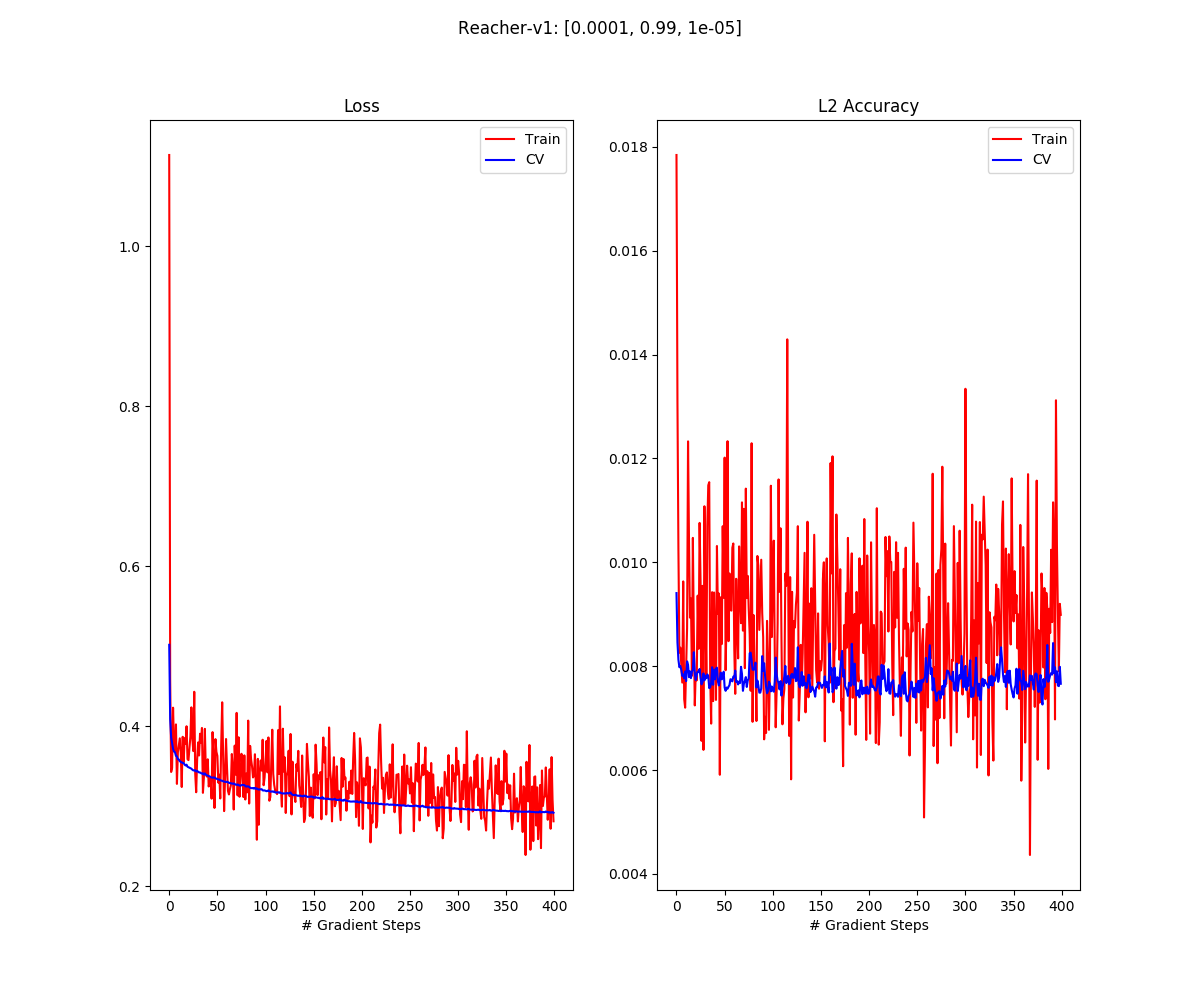
\includegraphics[scale=.6]{./images/reacher_train_summary.png}
\end{center}
For the Reacher environment over 20 rollouts the behavioral cloning agent recieved:\\
$\mathbb{E}[r]=-9.90198985254$\\
$\sigma(r) =  4.07604877598$\\
\\
The expert policy over 20 rollouts received:\\
$\mathbb{E}[r]=-3.75602940465$\\
$\sigma(r) =  1.51551772853$\\
\newpage
\begin{center}
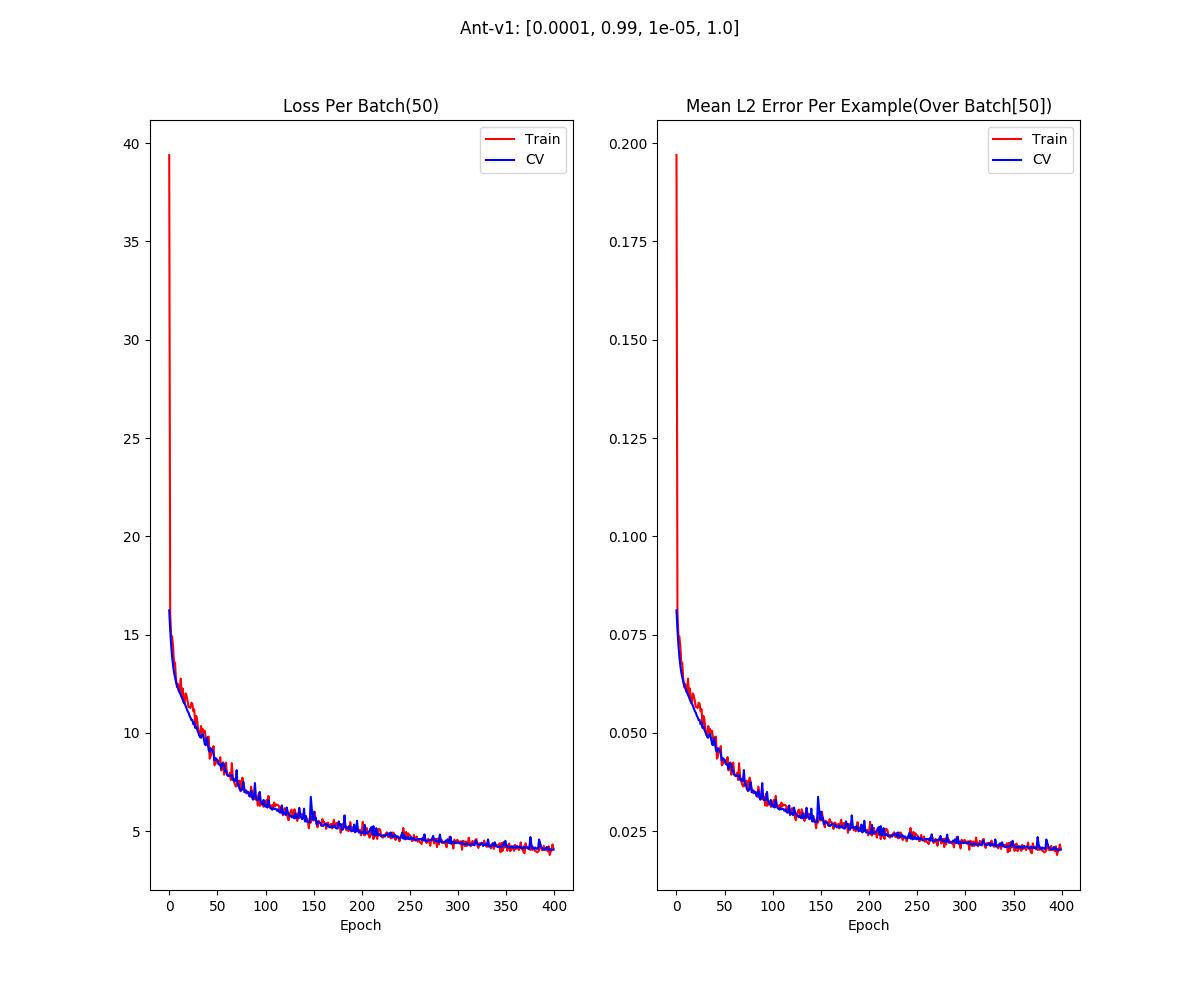
\includegraphics[scale=.6]{./images/ant_train_summary.png}
\end{center}
For the Ant environment over 20 rollouts the behavioral cloning agent received:\\
$\mathbb{E}[r]=1020.96629457$\\
$\sigma(r) =   36.176382481$\\
\\
The expert policy over 20 rollouts received:\\
$\mathbb{E}[r]=4633.75874581$\\
$\sigma(r) =   768.526309702$\\
\subsection*{2}
I decided to test dropout on my behavioral cloning model for the Reacher environment. The model architecture is 3 fully connected layers size 64, 64, 7 (with relu activations) as well as an input layer  size 11 and an output layer size 2. Between the last fully connected layer and the output sits a dropout layer with tuneable probability of dropout. I varied the keep propability (1-dropout probability) in increments of .025 from .7 to 1 and plotted the change in mean and standard deviation on the Reacher task across 20 rollouts.
\begin{center}
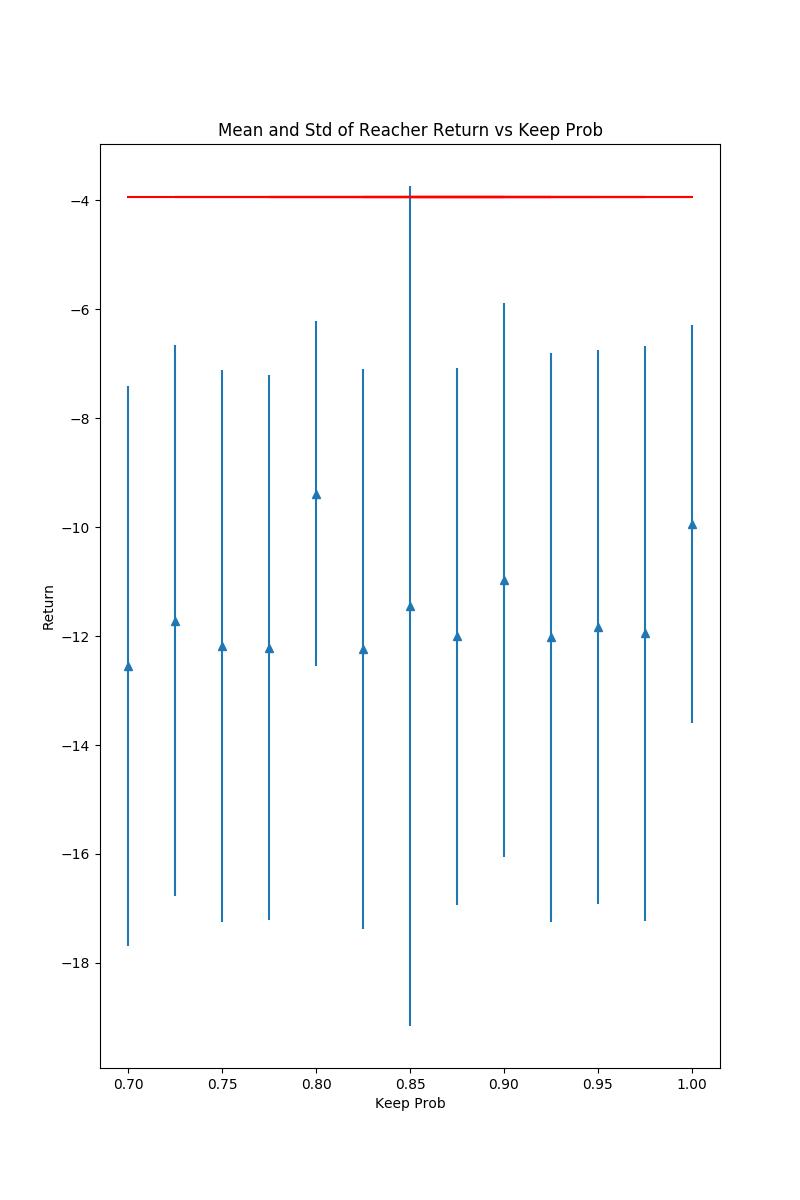
\includegraphics[scale=.5]{./images/2_2.png}
\end{center}
As stated earlier For the Reacher environment over 20 rollouts the behavioral cloning agent recieved:\\
$\mathbb{E}[r]=-9.90198985254$\\
$\sigma(r) =  4.07604877598$\\
\\

Keep probability of 1 (no dropout) achieved results closest to the expert policy so I decided to use 1 for this hyperparameter, essentially removing dropout from my network.
\end{document}